% mainfile:main.tex
% revised by dnolivieri
\chapter{Tab Groups}

\section{Analysis}

gedit presently uses a multiple document interface, called \emph{MDI}. By the use of tabs, it provides a way to visualize several documents in a single window. With the current interface,  gedit has the problem that it can not show different documents at the same time.  Indeed,  the only way that this can be performed at present is to open two gedit windows and resize them to fit the screen, which is very tedious and uncomfortable for the end user.

\subsection{Questions}


Given the problem described above, several more profound questions arise when brainstorming different implementation solutions: 
\begin{enumerate}
  \item How do we show the extra document to the user? Different tab groups or inside a tab?
  \item How do we want to allow the split? Vertically, Horizontally or allow both?
  \item How many side documents should we allow?
\end{enumerate}

\subsection{Do not reinvent the wheel}

In gereral, when analyzing a particular problem, the gedit development team passes through the following process: 
check what the competitors are doing, analyze their ideas,  and decide which of these ideas could best fit our requirements. 
Thus, before answering the specific questions posed above for multiple document tabs, the following programs were analyzed:



\subsubsection{Netbeans}

Figure \ref{fig:NetbeansScreenshot} shows that this program allows several tab groups\footnote{By tab groups, we refer to the ability of grouping tabs in different groups that can be viewed at the same time in a window}, which can be grouped either horizontally and vertically. This is due to the fact that netbeans uses a docking system which allows it to place the tabs whichever the user prefer. In GTK+ there is not such widget or facility that provide this capability.  There is, however, another library called \emph{GDL},  that provides this and it is used by programs like anjuta.  However, the library has the problem that it is not very well maintained and it would produce problems in the future.

\subsubsection{Kate}

With respect to  kate,  as shown in Figure \ref{fig:KateScreenshot}, it does not have proper tabs as in gedit, but instead usses a side pane showing the documents and it allows the user to open the documents either vertically or horizontally. This solution is outside the document tabbing design philosophy of gedit and can complicate teh discoverability for the end user.

\subsubsection{Notepad++}

In Figure \ref{fig:NotepadScreenshot}, we can see that Notepad++ it has a similar interface to that of gedit. It allows the user to create only one more tab group and it only makes an horizontally split.

\newpage
\addfigure[scale=0.29]{./images/netbeans}{Netbeans screenshot}{fig:NetbeansScreenshot}

\addfigure[scale=0.29]{./images/kate}{Kate screenshot}{fig:KateScreenshot}

\newpage
\addfigure{./images/notepad}{Notepad screenshot}{fig:NotepadScreenshot}

\subsection{Answering to the questions}

\begin{enumerate}
  \item Tab groups fit better into the  current gedit design, it will make it easier to use for the end user, and it will be easier to implement.
  \item Horizontal splits makes sense for visualizing documents side by side. Vertical split makes more sense if you are editing the same document in different parts of it. I.e having splitted the document to edit and show several parts of it.
  \item It was decided to allow n splits. It is up to the user to decide how many splits he wants. If in the future, restrictions are required, 
then it would be easier to impose them.
\end{enumerate}

\newpage

\section{Design}

\subsection{Prototyping}

In Figure \ref{fig:TabGroupsProto1},   prototype made with glade is shown in relation how it would look and what kind of widgets will be used. 
In Figure \ref{fig:TabGroupsProto2},  a prototype is shown that was made in order to answer the questions above, showing the vertical split. 
Apart from the visual design, the following points must be taken into account:
\begin{enumerate}
  \item By default, a gedit window has a single tab group (current behavior).
  \item The same document can NOT appear in different tab groups or different tabs.
\end{enumerate}

\begin{figure}[H]
  \begin{minipage}[b]{0.5\linewidth}
    \centering
    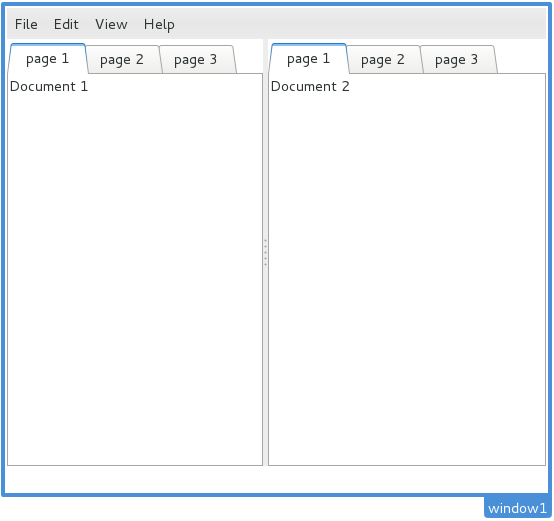
\includegraphics[scale=0.40]{./images/tab-groups-proto-1}
    \caption{Tab groups prototype 1}\label{fig:TabGroupsProto1}
  \end{minipage}
  \hspace{0.5cm}
  \begin{minipage}[b]{0.5\linewidth}
    \centering
    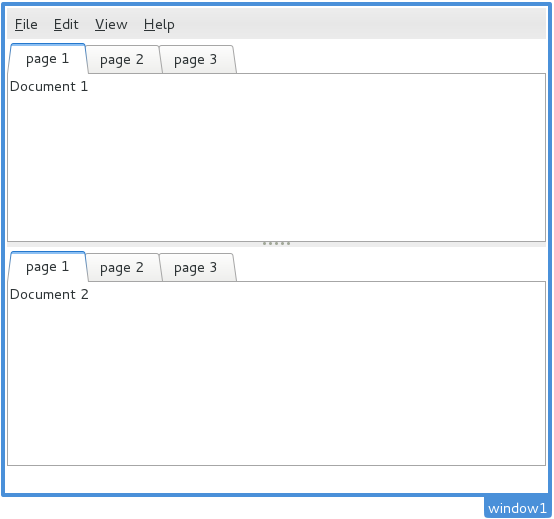
\includegraphics[scale=0.40]{./images/tab-groups-proto-2}
    \caption{Tab groups prototype 2}\label{fig:TabGroupsProto2}
  \end{minipage}
\end{figure}

\subsection{User interface}

In order to interact with tab groups, it was decided to provide three new menu items in the \emph{Documents} menu.
\begin{itemize}
  \item \textbf{New Tab Group:} It creates a tab group in the right of the focused one, and it adds a new tab to it.
  \item \textbf{Previous Tab Group:} Moves the focus to the previous (left) tab group.
  \item \textbf{Next Tab Group:} Moves the focus to the next (right) tab group.
\end{itemize}

\newpage
\subsection{Class diagram modification}

\addfigure[scale=0.45]{./images/tab-groups-diagram}{Tab groups diagram}{fig:TabGroupDiagram}

As it can be seen in Figure \ref{fig:TabGroupDiagram}, a new class has been introduced, \emph{GeditMultiNotebook}. This class will take care of create and remove GeditNotebooks, proxying the signals emittion for page-added, page-removed and switch-page and it will be kept as an implementation detail where the user will not have direct access to its API.

\newpage
\subsection{GeditMultiNotebook}

This class works as a proxy to \emph{GeditNotebook}, most of the API and signals are the same, here will be explained the different methods and signals.

\subsubsection{Signals}

\begin{table}[H]
  \begin{center}
    \begin{tabularx}{\textwidth}{|l|X|}
      \firsthline
      \textbf{Signal name:} & \textbf{Explanation:} \\
      \hline
      \textit{notebook\_added} & emitted when a new notebook has been added. \\
      \hline
      \textit{notebook\_removed} & emitted when a notebook is removed. \\
      \hline
      \textit{tab\_added} & proxy signal for page\_added from GtkNotebook. \\
      \hline
      \textit{tab\_removed} & proxy signal for page\_removed from GtkNotebook. \\
      \hline
      \textit{switch\_tab} & proxy signal for switch\_page from GtkNotebook. \\
      \hline
      \textit{tab\_close\_request} & proxy signal for tab\_close\_request from GeditNotebook. \\
      \hline
      \textit{page\_reordered} & proxy signal for page\_reordered from GtkNotebook. \\
      \hline
      \textit{show\_popup\_menu} & emitted when the right button of the mouse is clicked in the notebook. \\
      \lasthline
    \end{tabularx}
    \caption{Tab groups signals explanation}
  \end{center}
\end{table}

\begin{table}[H]
  \begin{center}
    \begin{tabularx}{\textwidth}{|l|X|}
      \firsthline
      \textbf{Method name:} & \textbf{Explanation:} \\
      \hline
      \textit{get\_active\_notebook} & Gets the active notebook, in order to know which one is the active, a track on the focused widget has to be taken. For this can be listened to the signal \emph{set-focus-child}. \\
      \hline
      \textit{get\_n\_notebooks} & Gets the number of notebooks, at least there will be one. \\
      \hline
      \textit{get\_nth\_notebook} & Gets the n notebook of the list. \\
      \hline
      \textit{get\_notebook\_num} & Given a notebook get the number in the list. \\
      \hline
      \textit{get\_n\_tabs} & Returns the number of tabs in all the notebooks. \\
      \hline
      \textit{get\_page\_num} & Finds the index of the page which contains the given tab. \\
      \hline
      \textit{get\_active\_tab} & Gets the active tab. \\
      \hline
      \textit{set\_active\_tab} & Sets the active tab. \\
      \textit{set\_current\_page} & Sets the active tab in relation to the total pages. \\
      \hline
      \textit{get\_all\_tabs} & Gets all the tabs. \\
      \hline
      \textit{close\_tabs} & Closes a list of tabs. \\
      \hline
      \textit{close\_all\_tabs} & Closes all tabs. \\
      \lasthline
    \end{tabularx}
  \end{center}
\end{table}

\newpage
\begin{table}[H]
  \begin{center}
    \begin{tabularx}{\textwidth}{|l|X|}
      \firsthline
      \textit{add\_new\_notebook} & Adds a new notebook. \\
      \hline
      \textit{remove\_active\_notebook} & Removes the active notebook. \\
      \hline
      \textit{previous\_notebook} & Focuses the previous notebook. \\
      \hline
      \textit{next\_notebook} & Focuses the next notebook. \\
      \lasthline
    \end{tabularx}
    \caption{Tab groups methods explanation}
  \end{center}
\end{table}

GTK+ provides a widget called \emph{GtkHPaned}, which is a container with two children arranged horizontally. An intensive use of this widget is needed in order to arrange the tab groups side by side.

The following pseudocode shows how it must be implemented:
\begin{lstlisting}[style=GObject]

void
add_notebook(new_notebook, main_container)
{
	if (main_container)
		main_container(new_notebook)
	else {
		paned = new_paned()
		parent = active_notebook.get_parent()
		parent.remove(active_notebook)
		parent.add(paned)

		paned.add1(active_notebook)
		paned.add2(new_notebook)
	}
	/* keep track of it in a list */
	notebooks.append(new_notebook)

	emit(notebook-added)
}

void
remove_notebook (notebook)
{
	if (notebooks.next() != NULL)
	{
		warning("Removing main notebook is not possible)
		return
	}

	ref(notebook)
	notebook.destroy()

	next = notebooks.next()
	parent = notebook.parent()
	children = parent.get_children()
	if (!children.next())
	{
		warning("parent must be a GtkPaned")
		return
	}

	grandpa = parent.parent()
	parent.remove(children[0])
	parent.destroy()
	grandpa.add(children[0])
	emit (notebook-removed, notebook)
	unref(notebook)
	focus(next)
}

\end{lstlisting}

\newpage
\section{Implementation}

To implemented this, there was one thing depending directly on GeditNotebook. \emph{GeditDocumentsPanel} (see figure \ref{fig:GeditDocumentsPanel1}), which shows in the side panel the currently opened documents and allows to manage them. This feature was disabled in order to be able to start the implementation.

\addfigure[scale=0.60]{./images/gedit-documents-panel1}{Documents panel}{fig:GeditDocumentsPanel1}

\subsection{Bugs}

In the next links,  the patches provided and the revisions by the other developers can be studied.

\noindent\url{https://bugzilla.gnome.org/show_bug.cgi?id=619608} \\
\noindent\url{https://bugzilla.gnome.org/show_bug.cgi?id=620502}

\newpage
\section{Tests}

\begin{table}[H]
  \begin{center}
    \begin{tabularx}{\textwidth}{|X|X|l|}
      \firsthline
      \textbf{Test:} & \textbf{Expected result:} & \textbf{Test passed?} \\
      \hline
      Click on new tab group & Adds a new tab group, and a new document on it & Yes \\
      \hline
      Close last tab & Closes the latest tab and removes the tab group & Yes \\
      \hline
      Click on previous tab group & Moves to the previous tab group & Yes \\
      \hline
      Click on next tab group & Moves to the previous tab group & Yes \\
      \hline
      Drag and drop between tabs & Allows to move a tab between tab groups & Yes \\
      \hline
      Change tab group & Reflects the active tab group in the documents menu, setting the shortcuts to the active one & Yes \\
      \lasthline
    \end{tabularx}
    \caption{Tests tab groups}
  \end{center}
\end{table}
